\documentclass[11pt]{article}
\usepackage[utf8]{inputenc}
\usepackage[T1]{fontenc}
\usepackage{lmodern}
\usepackage{microtype}
\usepackage{geometry}
\usepackage{graphicx}
\usepackage{booktabs}
\usepackage{amsmath,amssymb,amsthm}
\usepackage{xcolor}
\usepackage{hyperref}
\usepackage{enumitem}
\usepackage{caption}
\usepackage{subcaption}

\geometry{margin=1in}
\hypersetup{colorlinks=true, linkcolor=blue!50!black, urlcolor=blue!50!black, citecolor=blue!50!black}
\captionsetup{font=small, labelfont=bf}
\captionsetup[sub]{font=small}

\newtheorem{proposition}{Proposition}
\theoremstyle{definition}
\newtheorem{definition}{Definition}

\title{\textbf{Unknown Is Not Risky:\\Creative Decision Making with Calibrated Decision Models}}
\author{Chris Kagabe \& Archymedes \\[6pt]
\small \texttt{cdm} v0.2.0 --- exact decision theory on calibrated beliefs}
\date{October 2026}

\begin{document}

\maketitle

\begin{abstract}
Decision models select; they do not generate. We present \texttt{cdm}, a three-layer system that
keeps generation (people or a generative model write the options) separate from selection
(typed, calibrated judgments plus decision rules you control in code). The \emph{belief layer}
debiases, calibrates and pools judge outputs in Aitchison geometry; the \emph{value layer}
computes expected utility, CVaR, a fair-tie $P(\mathrm{best})$, expected improvement and EVPI on
finite lotteries; the \emph{policy layer} gates each option as clear, verify or reject and then
chooses to commit, reserve an innovation slot, spread a portfolio, or escalate.

The central design principle is that \emph{uncertainty is not, by itself, a reason to reject}:
an uncertain option is sent to a bounded check with a fallback to the status quo instead of being
vetoed. We make this precise. For a single decision, the value of a check depends on the belief
about the violation probability only through its mean, so ignorance and a known coin flip warrant
the same action; the difference matters for learning across decisions. We model imperfect checks
(sensitivity, specificity, cost, undetected harm), so residual risk is computed rather than assumed
away, and give a maximin rule over every dependence between checks. Every property is derived with
its hypotheses; doing so corrected two over-claimed properties and a tie-handling bug that the
tests had missed.

The evidence is kept apart by kind. (i) \emph{Implementation}: 88 property-based tests and oracles
at $99\%$ branch coverage, and agreement with Monte Carlo. (ii) \emph{A synthetic benchmark} with
$\tau$ chosen on held-out problems: checking uncertain options beats vetoing them (regret $0.045$
vs.\ $0.091$, paired gain $[0.041,0.050]$) at about $1\%$ undetected harm, against $17$--$23\%$ for
acting on them unchecked. The gain holds under worse checks and a confidently wrong judge, but it
comes from checking, not from the CVaR reliability gate, which the best policy leaves unbound.
(iii) \emph{A semi-synthetic benchmark with 237 real Jev calls} and ground truth by construction:
Jev separates explicit harm from explicit safety almost perfectly (AUROC $0.9998$), is
calibrated on average on ambiguous options but varies with phrasing, and is more overconfident on
value than its audit prior assumes. Over 48 problems \texttt{cdm} has the lowest regret and harm
(gain over veto $0.051$, bootstrap interval $[0.009,0.102]$), with a gain that depends on an assumed
status-quo value. None of this establishes better decisions on real outcomes, which we specify as
the main open problem.
\end{abstract}

\noindent\textbf{Keywords:} calibrated decision models, decision theory, Aitchison geometry,
CVaR, value of information, verification, position bias

\tableofcontents
\newpage

% ==============================================================================================
\section{Introduction}

A creative decision is a choice among options none of which is provably best. The interesting
options are \emph{novel}: there is little precedent, so little historical frequency to learn from,
and the decision must rest on judgment. Much current tooling asks one model to propose an option,
justify it and approve it. That conflates divergence (inventing options) with convergence
(choosing one). A model that writes a persuasive rationale is not thereby calibrated: judgment
models are often overconfident, sensitive to presentation order, and unable to say ``I do not
know'' in a way a program can act on.

We separate the jobs. People or a generative model diverge; a pipeline of typed judgments
converges through decision rules stated as math and checked by tests:
\begin{equation*}
\scalebox{0.92}{$\text{options} \times \text{judges}
\;\xrightarrow{\text{belief}}\;
\Delta^\circ(\text{levels})^{D}
\;\xrightarrow{\text{value}}\;
\mathrm{Lotteries}(\mathbb{R})
\;\xrightarrow{\text{policy}}\;
(\text{commit}, \text{innovate}, \text{portfolio}, \text{escalate}).$}
\end{equation*}

\paragraph{The principle, stated carefully.} The slogan in our title is shorthand for a narrower
claim: \emph{uncertainty is not, by itself, a reason for automatic rejection}. If an option can be
checked cheaply, with a working fallback, then an unfamiliar option should be checked rather than
vetoed, so the system can be conservative about irreversible commitment without being
conservative about exploration. Two caveats are central and are developed in
\S\ref{sec:uncertainty}. First, a point estimate $q=0.5$ cannot tell ``we do not know'' from ``we
know the harm rate is one half''; only the former is a reason to verify. Second, the downside is
bounded only as well as the check works: a check that misses violations leaves residual risk,
which we now model explicitly.

\paragraph{Contributions.}
\begin{enumerate}[leftmargin=1.6em,itemsep=1pt]
\item An architecture that makes selection a separate, inspectable process: judgments enter as
calibrated distributions, and the decision rule is ordinary code with stated properties
(\S\ref{sec:layers}).
\item A gate-and-fallback policy (clear / verify / reject, commit / innovate / portfolio /
escalate) with properties P1--P8 derived under stated hypotheses, an explicit model of imperfect
verification, the value of a one-shot check, and a maximin rule over dependence between checks
(\S\ref{sec:uncertainty}, Appendix~\ref{app:proofs}).
\item An implementation whose claims are mapped to property-based tests; a synthetic benchmark with
held-out tuning, ablation and robustness checks; and a benchmark that runs the policy on real Jev
judgments against known ground truth (\S\ref{sec:experiments}).
\end{enumerate}
The mathematical components are established; the contribution is their integration into one
decision policy, and a clear account of what that policy does and does not guarantee.

% ==============================================================================================
\section{Related work}

\emph{Calibration.} Temperature and Platt scaling correct systematic over- or under-confidence
\cite{platt1999,guo2017}; they do not say how to act, and calibration measured in aggregate can hide
miscalibration in sub-populations. \emph{Combining judges.} Linear and logarithmic opinion pools
\cite{genest1986} combine distributions; the log pool is externally Bayesian, but neither pool
corrects for correlated errors. \emph{Compositional data.} Aitchison geometry makes the open
simplex a vector space \cite{aitchison1986}, which turns calibration, pooling and Bayes updates into
linear operations. \emph{Presentation bias.} LLM judges are sensitive to option order
\cite{zheng2024}; permuting and averaging is the standard mitigation, and we state when it is exact.
\emph{Risk.} Coherent risk measures \cite{artzner1999} and CVaR \cite{rockafellar2000} quantify
downside for a given distribution. \emph{Exploration and information.} Expected improvement
\cite{jones1998} trades exploration against exploitation; the value of information
\cite{howard1966} prices further inquiry; conservative bandits \cite{wu2016} explore while keeping
performance close to a baseline, which is close in spirit to our reliability gate. Online weights
use Hedge \cite{freund1997}.

% ==============================================================================================
\section{The three layers}\label{sec:layers}

\begin{figure}[t]
\centering
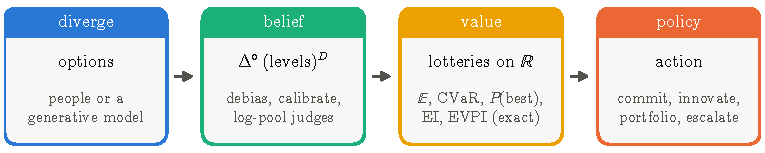
\includegraphics[width=\linewidth]{paper_figs/fig_pipeline}
\caption{Generation is kept apart from selection. The belief layer turns judge outputs into
calibrated distributions over levels; the value layer turns them into finite lotteries; the policy
layer gates and selects. An option that fails verification falls back to the status quo $B$.}
\label{fig:pipeline}
\end{figure}

\subsection{Belief layer: Aitchison geometry on the simplex}\label{sec:belief}

Raw model output can contain exact 0s and 1s, on the boundary of the simplex where log-ratios
break. The one non-linear step, \texttt{interior}$(p,\eta)=(1-\eta)p+\eta u$, moves it into the
open simplex $\Delta^\circ_K=\{p: p_i>0,\ \sum p_i=1\}$. On $\Delta^\circ$ define perturbation
$p\oplus q = C(p\cdot q)$ (the closure $C$ rescales to sum 1), powering $\alpha\odot p=C(p^\alpha)$,
and the centred log-ratio $\mathrm{clr}(p)=\log p-\overline{\log p}$, a linear isomorphism onto
$\{x:\sum x=0\}$. Every belief operation below is linear in clr coordinates
(Table~\ref{tab:belief-ops}, Figure~\ref{fig:belief}).

\begin{table}[h]
\centering\small
\begin{tabular}{@{}lll@{}}
\toprule
operation & formula & meaning \\
\midrule
Bayesian update & $\ell\oplus p$ & evidence likelihood $\ell$ \\
temperature calibration & $(1/T)\odot p$ & correct over-/under-confidence \\
log opinion pool & $\bigoplus_j (w_j\odot p_j)$ & combine judges \\
orbit debiasing & $\frac1{|G|}\odot\bigoplus_g g^{-1}\cdot p_g$ & cancel position bias \\
\bottomrule
\end{tabular}
\caption{Belief operations are linear in Aitchison geometry; only \texttt{interior} is not.}
\label{tab:belief-ops}
\end{table}

\textbf{B1 (tempering is a group action).} $\beta_1\odot(\beta_2\odot p)=(\beta_1\beta_2)\odot p$,
$1\odot p=p$; ranking is preserved for $\beta>0$; $T\to\infty$ gives uniform.
\textbf{B2.} The calibration NLL is convex in $\beta=1/T$, so a one-dimensional search finds the
global optimum. \textbf{B3.} The pool is symmetric in judges, unanimous when $\sum w=1$, and
satisfies $\mathrm{pool}(\ell\oplus p_j)=(\sum w)\odot\ell\oplus\mathrm{pool}(p_j)$, i.e.\ it is
externally Bayesian exactly when $\sum w=1$. \textbf{B4.} If the judge's bias is
\emph{multiplicative in position}, a transitive cyclic orbit $Z_n$ removes it exactly; under
reversal $Z_2$ (the only non-trivial re-ordering that keeps an ordinal scale ordinal) the odd part
of $\mathrm{clr}(\mathrm{bias})$ cancels and the even part remains. Exactness holds for the raw
answers. The pipeline first applies \texttt{interior} with $\eta>0$, which is not multiplicative,
so with the default $\eta=0.03$ the cyclic orbit is only approximately unbiased
(\S\ref{sec:biasrec} quantifies the error). Bias that interacts with content is only reduced. \textbf{B5.} Hedge weights $w\propto e^{-\eta\,\mathrm{loss}}$ are shift-invariant
and antitone in loss. Derivations are in Appendix~\ref{app:proofs}.

\begin{figure}[t]
\centering
\begin{subfigure}[t]{0.48\linewidth}
\centering
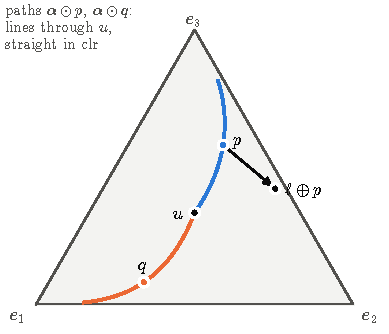
\includegraphics[width=\linewidth]{paper_figs/fig_simplex}
\caption{The open 2-simplex. Tempering paths $\alpha\odot p$ are straight lines through the
uniform point $u$ in clr coordinates; a Bayes update $\ell\oplus p$ is a translation.}
\end{subfigure}\hfill
\begin{subfigure}[t]{0.48\linewidth}
\centering
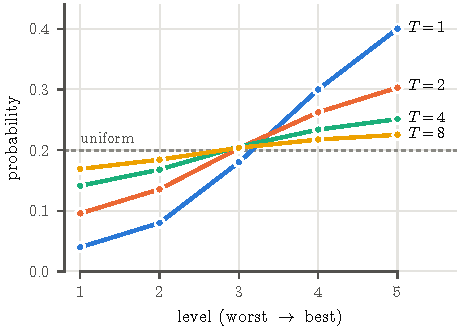
\includegraphics[width=\linewidth]{paper_figs/fig_temper}
\caption{Tempering an overconfident five-level belief: larger $T$ moves it toward uniform while
preserving the ranking of levels.}
\end{subfigure}
\caption{Belief layer: Aitchison geometry and calibration.}
\label{fig:belief}
\end{figure}

\subsection{Value layer: finite lotteries}\label{sec:value}

A lottery $\mu=\sum_k p_k\,\delta_{x_k}$ has sorted, distinct atoms and masses summing to 1. Binary
operations combine \emph{independent} copies, so $X+X$ is a convolution, not $2X$.

\paragraph{What ``exact'' means.} All functionals are computed by enumeration, with no sampling,
\emph{for the lottery that is represented}. That lottery is a model: it inherits the judges'
calibration, the chosen level utilities, and the independence assumptions. And when a convolution
would exceed 4096 atoms it is compacted onto a grid, keeping mass and mean exactly but moving
quantiles and CVaR by up to one grid step. Exactness is therefore a property of the arithmetic,
not of the beliefs.

\paragraph{Definitions.} For a lottery $X$ with CDF $F$ and quantile function $F^{-1}$, the
lower-tail mean at level $\alpha\in(0,1]$ is
\begin{equation}
\mathrm{CVaR}_\alpha(X)=\frac1\alpha\int_0^\alpha F^{-1}(u)\,du
=\max_{t\in\mathbb R}\Bigl\{t-\tfrac1\alpha\,\mathbb E\bigl[(t-X)^+\bigr]\Bigr\},
\end{equation}
which takes the part of an atom that straddles the $\alpha$-quantile in proportion. Two values are
treated as equal when they differ by less than a relative $10^{-9}$: atoms that agree to that
tolerance are merged and count as ties in $P(\mathrm{best})$ and in the argmax. Without this, rounding
errors from different computation paths made equal values unequal; writing down P8 exposed the bug.

\textbf{L1.} $(+,\cdot)$ are commutative and associative; expectation is linear; variances add for
independent sums. \textbf{L2.} Lower-tail $\mathrm{CVaR}_\alpha$ is FSD-monotone,
translation-equivariant, positively homogeneous, superadditive, bounded by the mean, monotone in
$\alpha$, with $\mathrm{CVaR}_1=\mathbb{E}$. \textbf{L3.} Compaction preserves mass and mean and
moves CVaR by at most one grid step; a lottery built through $m$ compacting operations is within
the sum of their grid steps.

\textbf{L4 (fair-tie $P(\mathrm{best})$).} For independent competitors $V_j$, where competitor $j$
is removed (value $-\infty$) with probability $r_j$,
\begin{equation}
P(\mathrm{best}_i)
= \sum_x p_i(x)\int_0^1 \prod_{j\neq i}\bigl(F_j(x^-) + p_j(x)\,t\bigr)\,dt ,
\qquad \int_0^1 t^k\,dt = \frac{1}{k+1},
\end{equation}
which averages $1/(1+\#\text{ties})$ over the number of ties. It sums to 1, is
permutation-equivariant and splits equally between identical competitors
(Figure~\ref{fig:value}b). \textbf{L5.}
$\mathbb{E}[\max_j U_j]=\sum_x x\,\Delta\prod_j F_j(x)$ and $\mathrm{EVPI}=\mathbb{E}[\max_j
U_j]-\max_j\mathbb{E}[U_j]\ge 0$. \textbf{L6.} $\mathrm{EI}(V;B)=\mathbb{E}[\max(V-B,0)]$ is
monotone in the convex order (a mean-preserving spread never lowers it) and is at least the mean
gain (Figure~\ref{fig:policy}a).

\begin{figure}[t]
\centering
\begin{subfigure}[t]{0.48\linewidth}
\centering
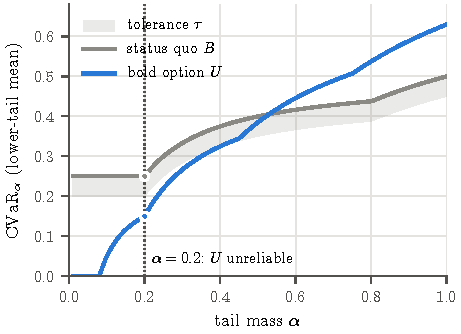
\includegraphics[width=\linewidth]{paper_figs/fig_cvar}
\caption{$\mathrm{CVaR}_\alpha$ of a bold option $U$ and the status quo $B$. At $\alpha=0.2$, $U$
falls below the band $[\mathrm{CVaR}(B)-\tau,\mathrm{CVaR}(B)]$, so it is not reliable, although
its mean is higher.}
\end{subfigure}\hfill
\begin{subfigure}[t]{0.48\linewidth}
\centering
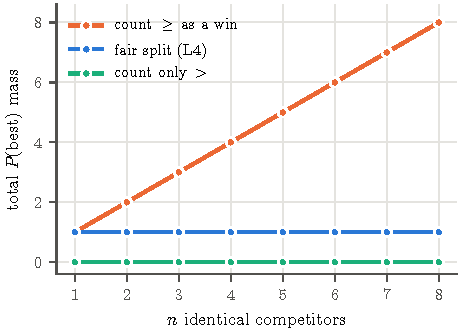
\includegraphics[width=\linewidth]{paper_figs/fig_ties}
\caption{Total $P(\mathrm{best})$ mass among $n$ identical competitors. Counting $\geq$ as a win
over-counts ($n$); counting only $>$ under-counts (0); the fair split of L4 sums to 1.}
\end{subfigure}
\caption{Value layer: the reliability test and fair tie splitting.}
\label{fig:value}
\end{figure}

\subsection{Policy layer: gates and selection}\label{sec:policy}

For option $i$ with dimension beliefs $p_{i,d}$, level utilities $v_d$, weights $w_d$, soft
penalties $\lambda$ and hard-violation probabilities $q_{i,c}$:
\begin{align*}
V_i &= m+\Bigl(\sum_d \frac{w_d}{\sum w}\,X_{i,d}-m\Bigr) \prod_{\text{soft }c} M_{i,c},
&& M_{i,c}=\begin{cases}1-\lambda &\text{w.p. }q_{i,c}\\1&\text{else}\end{cases}\\
f_i &= 1-\prod_{\text{hard }c}(1-q_{i,c}),
&& U_i=\begin{cases}V_i &\text{w.p. }1-f_i\\ B &\text{w.p. }f_i\end{cases}
\end{align*}
where $m=\sum_d\frac{w_d}{\sum w}\min v_d$ is the utility floor and $B$ is the status quo (the
baseline, or doing nothing). Soft penalties shrink utility toward the floor rather than toward
zero; in v0.1 they multiplied $V$ itself, so a penalty \emph{raised} utility whenever level values
were negative and decisions depended on where zero sat (P8 below). The second line is the
\emph{perfect-check} model; \S\ref{sec:verify} generalises it. A hard check is \textbf{clear}
($q\le\delta$), \textbf{verify} ($\delta<q<\rho$) or \textbf{reject} ($q\ge\rho$); defaults are
$\delta=0.15$, $\rho=0.7$.
\begin{align}
\text{reliable}(i) &\iff \mathrm{status}\neq\mathrm{reject}
\ \land\ \mathrm{CVaR}_\alpha(U_i)\ge \mathrm{CVaR}_\alpha(B)-\tau \\
\text{commit} &= \arg\max_{\text{reliable}}\ \mathbb{E}[U_i]
&& \text{ties}\to\text{status quo, then id} \\
\text{innovation} &= \arg\max_{\text{reliable},\ \mathrm{novelty}\ge\nu,\ \neq\text{commit}}
\ \mathrm{EI}_i \\
\text{portfolio} &= P(\mathrm{best})\text{ over }\{B\}\cup\{\text{best reliable per niche}\} \\
\text{escalate} &\iff \mathrm{EVPI}>\kappa .
\end{align}
Here $\mathrm{EI}_i=\mathbb E[(U_i-B)^+]$ \emph{with $U_i$ and $B$ coupled}: when option $i$ falls back,
its outcome is the same draw of $B$, so that branch contributes zero. In closed form, with
perfect checks $\mathrm{EI}_i=(1-f_i)\,\mathbb E[(V_i-B)^+]$ for independent $V_i,B$ (the general
form is in \S\ref{sec:verify}). Reading the formula with an independent copy of $B$ in the
fallback branch would credit an option for the status quo's own variance.
The reliability test allows $\mathrm{CVaR}_\alpha(U_i)$ to sit up to $\tau$ \emph{below} the status
quo's: it is a tolerance on tail loss, not a pointwise guarantee.

\textbf{Properties.} Each has a property-based test and a derivation in
Appendix~\ref{app:proofs}; the derivations fixed the statements of P2, P4, P6 and P7, which
earlier versions over-claimed.
\begin{itemize}[leftmargin=1.6em,itemsep=1pt]
\item[\textbf{P1}] The baseline is reliable, so a commit always exists; $P(\mathrm{best})$ and the
portfolio each sum to 1; EVPI $\ge0$.
\item[\textbf{P2}] Permuting options permutes the outputs. Renaming them does too, except that an
exact tie in $\mathbb E[U]$ between two non-baseline options goes to the smaller id.
\item[\textbf{P3}] Scaling all weights by $c>0$ changes nothing.
\item[\textbf{P4}] Adding a rejected option, or one whose $\mathbb{E}[U]$ is strictly below the
commit's, leaves the commit unchanged; exact ties go to the status quo, then to the smaller id.
\item[\textbf{P5}] Novelty only gates the innovation slot.
\item[\textbf{P6}] Raising a hard-violation probability never improves an option's status and never
lowers $f$. With perfect checks $\mathbb E[U]$ moves toward $\mathbb E[B]$; with imperfect checks and
$H\le\min B$, EI never rises. (With imperfect checks $\mathbb E[U]$ need \emph{not} move toward
$\mathbb E[B]$: the missed-harm branch can pull it below.)
\item[\textbf{P7}] With perfect checks, if $V_i\succeq_{\mathrm{FSD}}V_j$ and $f_i\le f_j$ then
$P(\mathrm{best}_i)\ge P(\mathrm{best}_j)$, and $\mathbb E[U_i]\ge\mathbb E[U_j]$ provided
$\mathbb E[V_j]\ge\mathbb E[B]$. Without that proviso the second claim is false: two options with the
same $V$ below a better status quo reverse, because the riskier one falls back more often.
\item[\textbf{P8}] Mapping every level value, $H$ and the null value by $x\mapsto ax+b$ ($a>0$), and
$\tau,\kappa,k$ by $x\mapsto ax$, maps every $\mathbb E$, CVaR and EI the same way and leaves every
gate state, $P(\mathrm{best})$, commit, innovation and escalation unchanged.
\end{itemize}

% ==============================================================================================
\section{Uncertainty, verification and dependence}\label{sec:uncertainty}

\subsection{Unknown versus risky}\label{sec:unknown}

A single number $q$ cannot carry the whole distinction the slogan suggests. Write the belief about
an option's violation probability as a distribution $\pi(q)$, for example $\mathrm{Beta}(a,b)$ with
mean $\bar q=a/(a+b)$ and concentration $n=a+b$. Figure~\ref{fig:unknown} shows complete ignorance
$\mathrm{Beta}(1,1)$ and a well-measured coin flip $\mathrm{Beta}(50,50)$, which share $\bar q=0.5$,
and evidence of harm $\mathrm{Beta}(18,2)$. It is tempting to say that only the first is a reason to
verify. For a single decision that is false.

\begin{proposition}[The value of a one-shot check depends on $\pi$ only through $\bar q$]
\label{prop:voc}
Let a check observe whether \emph{this} option violates, with sensitivity $s$, specificity $c$ and
cost $k$, and let a missed violation be worth $H$. Acting on the option after the check rather than
blindly changes expected utility by
\[
\Delta_{\text{check}}=\bar q\,s\,\bigl(\mathbb E[B]-H\bigr)-(1-\bar q)(1-c)\bigl(\mathbb E[V]-\mathbb E[B]\bigr)-k,
\]
and verifying beats rejecting (keeping $B$) if and only if
$(1-\bar q)\,c\,\bigl(\mathbb E[V]-\mathbb E[B]\bigr)>\bar q\,(1-s)\bigl(\mathbb E[B]-H\bigr)+k$.
Both depend on $\pi$ only through $\bar q=\mathbb E_\pi[q]$.
\end{proposition}

The check observes the event, and $P(\text{violation})=\mathbb E_\pi[q]$ by the tower rule; every
branch probability is affine in it. So ignorance and a known coin flip warrant the same gate state,
and \texttt{cdm} is right to act on $\bar q$ alone \emph{within one decision}. The shape of $\pi$
matters for \emph{learning}. When options share a mechanism, one checked outcome updates the belief
about the next one: under $\mathrm{Beta}(1,1)$ a single observation moves the mean from $0.5$ to
$0.67$ or $0.33$, while under $\mathrm{Beta}(50,50)$ it moves by $0.005$. Verification under
ignorance is therefore also an experiment, and its full value includes this information for future
decisions. Capturing that needs judges that report uncertainty about $q$, and a sequential policy
that keeps beliefs per mechanism. Both are outside v0.2.0.

There is an empirical point too. With a real judge, ``unknown'' options rarely sit at $q\approx0.5$:
on the ambiguous options of our Jev benchmark (\S\ref{sec:jev}) the median $q$ is about $0.3$, and
Jev's $q$ varies with phrasing even where the true rate does not.

\begin{figure}[t]
\centering
\begin{subfigure}[t]{0.48\linewidth}
\centering
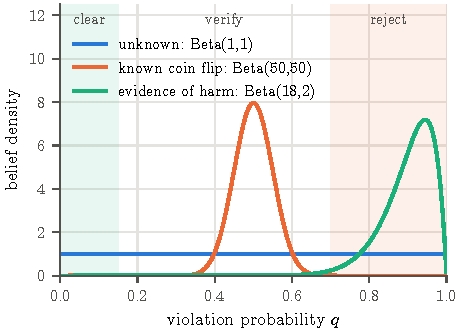
\includegraphics[width=\linewidth]{paper_figs/fig_unknown}
\caption{Ignorance and a known 50\% harm rate share $\bar q=0.5$, and so the same value of a
one-shot check (Proposition~\ref{prop:voc}). They differ in what a check teaches about similar
options.}
\label{fig:unknown}
\end{subfigure}\hfill
\begin{subfigure}[t]{0.48\linewidth}
\centering
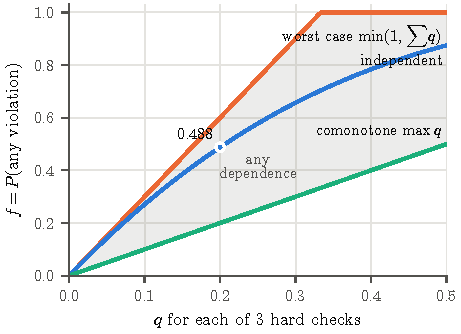
\includegraphics[width=\linewidth]{paper_figs/fig_dependence}
\caption{Three hard checks, each with violation probability $q$. Independence gives
$1-(1-q)^3$ (0.488 at $q=0.2$); without assumptions $f$ lies anywhere in the shaded band.}
\label{fig:dependence}
\end{subfigure}
\caption{The two assumptions behind the gate: what $q$ means, and how checks combine.}
\end{figure}

\subsection{Imperfect verification and residual risk}\label{sec:verify}

The perfect-check model assumes a check catches every violation, never raises a false alarm,
costs nothing and resolves before any exposure. We drop the first three assumptions. Let a check
have sensitivity $s=P(\text{caught}\mid\text{violation})$, specificity
$c=P(\text{pass}\mid\text{no violation})$ and cost $k$, and let $H$ be the utility of an undetected
violation. Then
\begin{equation}\label{eq:verify}
U_i=\begin{cases}
V_i - k & \text{w.p. } (1-f_i)\,c \quad\text{(passes, no violation)}\\
B - k & \text{w.p. } f_i\,s + (1-f_i)(1-c) \quad\text{(caught, or false alarm)}\\
H - k & \text{w.p. } f_i\,(1-s) \quad\text{(missed)}
\end{cases}
\end{equation}
with $k$ charged to options in the verify state. The defaults $s=c=1$, $k=0$ recover the
perfect-check model exactly. As in the perfect-check model, the fallback applies to every hard
constraint, including those in the clear state (which are assumed monitored at no explicit cost);
a constraint that is not actually monitored should be modelled with $s=0$. The policy layer needs only $U_i$, the race entry for $P(\mathrm{best})$ (the fallback branch is
removed from the race, since it \emph{is} the status-quo action) and
\[
\mathrm{EI}_i=(1-f_i)c\;\mathbb E\bigl[(V_i-k-B)^+\bigr]+f_i(1-s)\;\mathbb E\bigl[(H-k-B)^+\bigr],
\]
with $V_i$ and $B$ independent inside each expectation; the fallback branch contributes nothing.

\begin{proposition}[What the fallback does and does not bound]\label{prop:downside}
Under \eqref{eq:verify}, for any threshold $x$,
\[
P(U_i < x) \;=\; (1-f_i)c\,P(V_i<x+k) + \bigl(f_i s + (1-f_i)(1-c)\bigr)P(B<x+k) + f_i(1-s)\,\mathbf{1}[H<x+k].
\]
In particular, with $k=0$ and $x=\min B$: $P(U_i<\min B)=(1-f_i)c\,P(V_i<\min B)+f_i(1-s)\,\mathbf 1[H<\min B]$.
The fallback removes the failure branch from the downside only when $s=1$; the residual risk is
$f_i(1-s)$; and the passing branch always carries $V_i$'s own lower tail, which the policy controls
only through $\mathrm{CVaR}_\alpha(U_i)\ge\mathrm{CVaR}_\alpha(B)-\tau$.
\end{proposition}

So the earlier informal claim ``verify bounds the downside by construction'' is true in a narrow
sense: with a perfect check, the \emph{failure} branch lands exactly on $B$. It is not a guarantee
that realised outcomes are at least as good as the status quo. Figure~\ref{fig:policy}b shows the
utility distribution of a bold option as sensitivity falls. Three questions remain outside the
model and must be answered per application: whether exposure can occur \emph{before} the check
resolves, whether the fallback is itself available and reliable, and how $s$, $c$ and $H$ are
estimated.

\begin{figure}[t]
\centering
\begin{subfigure}[t]{0.48\linewidth}
\centering
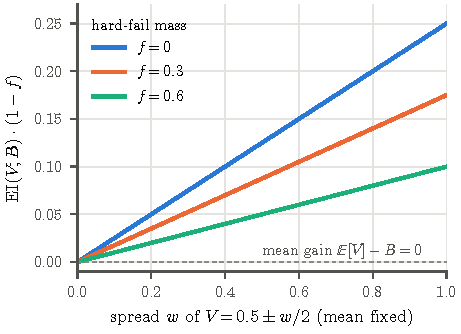
\includegraphics[width=\linewidth]{paper_figs/fig_ei}
\caption{Expected improvement over a fixed $B=0.5$ for a mean-preserving spread
$V=0.5\pm w/2$. EI rises linearly with spread and is scaled down by the hard-fail mass $f$.}
\end{subfigure}\hfill
\begin{subfigure}[t]{0.48\linewidth}
\centering
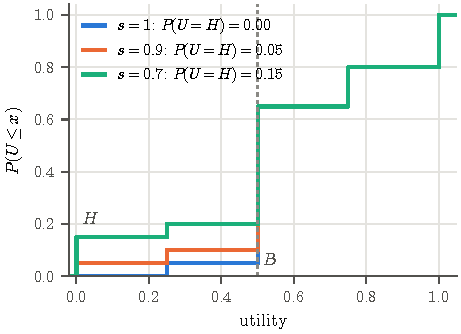
\includegraphics[width=\linewidth]{paper_figs/fig_verify}
\caption{CDF of $U$ for a bold option with $f=0.5$ and $B=0.5$. With a perfect check ($s=1$) no
mass falls to $H=0$; at $s=0.9$ and $0.7$, mass $f(1-s)$ does. Curves coincide above $B$.}
\end{subfigure}
\caption{Policy layer: innovation rewards spread, and the fallback is only as good as the check.}
\label{fig:policy}
\end{figure}

\subsection{Dependence between checks and between judges}\label{sec:dependence}

The failure mass $f_i=1-\prod_c(1-q_{i,c})$ assumes independent checks. For three checks at
$q=0.2$ that gives $0.488$; but without any assumption the Fr\'echet bounds give
\begin{equation}
\max_c q_{i,c}\;\le\; f_i \;\le\; \min\Bigl(1,\sum_c q_{i,c}\Bigr),
\end{equation}
i.e.\ anywhere in $[0.2,0.6]$ (Figure~\ref{fig:dependence}). Using the upper bound is \emph{not} a
worst case for the decision: with $B$ better than $V$, a larger $f$ raises $\mathbb E[U]$, and a
larger $f$ can also raise CVaR (\S\ref{sec:spread}). \texttt{cdm} instead offers
\texttt{hard\_dependence="robust"}: since every branch weight in \eqref{eq:verify} is affine in $f$,
$\mathbb E[U_i]$ is affine in $f$, so its minimum over all dependence structures is attained at one
of the two ends, and the policy evaluates both and keeps the worse. This is a maximin rule for
expected utility. CVaR is then computed at that $f$; it is not separately minimised (as a function of
the mixing weight it is convex, so its minimum can be interior). Gate states depend only on the
marginal $q_{i,c}$ and do not change. Positive dependence (one root cause behind several violations)
moves $f_i$ \emph{down} toward $\max_c q_{i,c}$, so independence is not automatically conservative
either. A single sensitivity $s$ is applied to the union of all hard checks; per-check
sensitivities would need the joint law of the violations.

Dependence between judges is harder. With $\sum w=1$ the log pool is a weighted geometric mean, so
pooling $m$ copies of the same judge returns that judge: the pool does not over-count agreement.
But it also cannot detect that two different judges share a blind spot. If both rate a whole style
of idea too highly, the pooled belief inherits the error with full confidence. We do not model
this; the mitigation is to pool judges that differ in training data and architecture, and to
measure their error correlation on held-out outcomes before trusting the pool.

\subsection{The innovation slot and the incentive toward spread}\label{sec:spread}

The innovation candidate maximises expected improvement over $B$, which by L6 rewards spread. That
is intended, since a novel idea's value is often in its upper tail, but it is also an incentive to
favour volatility, so the reliability gate is what keeps it in check. Figure~\ref{fig:innovation}
sweeps a two-option problem: a \emph{narrow} option and a \emph{wide} one with the same mean, both
novel, against a status quo with a slightly higher mean (so the status quo stays the commit).

\begin{figure}[t]
\centering
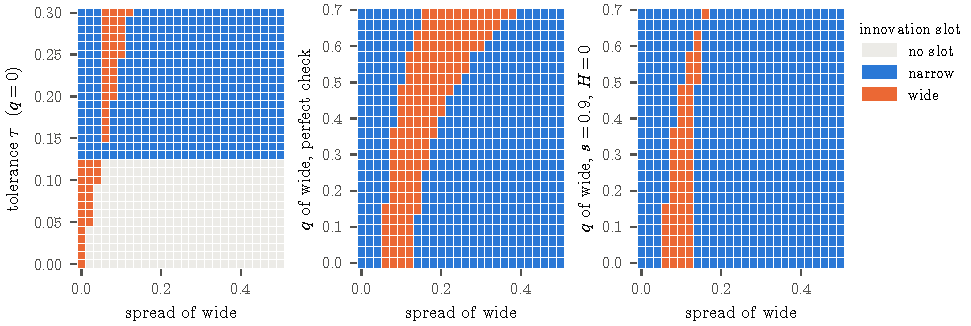
\includegraphics[width=\linewidth]{paper_figs/fig_innovation}
\caption{Which option takes the innovation slot (narrow and wide have equal means; both are
novel). Left: as spread grows, the wide option's CVaR falls and it is excluded unless $\tau$ is
large; at small $\tau$ nothing qualifies. Middle ($\tau=0.3$, perfect check): a \emph{higher}
violation probability lets \emph{wider} options pass, because failures land on $B$ and lift the
tail. Right (same, with $s=0.9$, $H=0$): pricing missed violations removes that artifact.}
\label{fig:innovation}
\end{figure}

Three observations follow. First, spread wins only inside a bounded region: past a spread set by
$\tau$, the wide option fails the reliability test and the slot goes to the narrow one, so the
policy does not reward volatility without limit. Second, the perfect-check model contains a
perverse incentive: raising $q$ turns more of the wide option's lower tail into the status quo,
which raises its CVaR, so a \emph{riskier} volatile option can look \emph{more} reliable (middle
panel). Third, the imperfect-check model of \S\ref{sec:verify} removes it: with $s=0.9$ each unit
of $q$ also adds mass at $H$, and the region where the wide option wins no longer grows with $q$
(right panel). We therefore recommend the check model whenever $q$ is material, even with a rough
estimate of $s$.

% ==============================================================================================
\section{Experiments}\label{sec:experiments}

\subsection{What each piece of evidence supports}

We report six kinds of evidence. Table~\ref{tab:evidence} states what each supports and what it
does not; only the two benchmarks compare decision rules, and only the second uses a real judge.

\begin{table}[h]
\centering\small
\setlength{\tabcolsep}{4pt}
\begin{tabular}{@{}p{0.27\linewidth}p{0.335\linewidth}p{0.335\linewidth}@{}}
\toprule
evidence & supports & does not establish \\
\midrule
property tests, oracles, derivations & the code implements the stated formulas, which hold under
their stated hypotheses & that the formulas describe the world \\
exact vs.\ Monte Carlo & two implementations agree on the represented lottery & that the lottery
is accurate \\
synthetic bias recovery & the pipeline removes a planted multiplicative bias & that real biases have
that form \\
live Jev run & the pipeline works end to end on a real API & better decisions than alternatives \\
synthetic policy benchmark & how the gates trade regret against harm when the world matches the
model & behaviour when it does not \\
Jev benchmark (\S\ref{sec:jev}) & how the policy performs on a real judge's judgments when the truth is known by construction &
performance on real decisions and real outcomes \\
\bottomrule
\end{tabular}
\caption{Evidence and its limits.}
\label{tab:evidence}
\end{table}

\subsection{Implementation: property-based tests and oracles}

Every numbered claim has a property-based test (Hypothesis); L4/L5 also have a brute-force oracle
over joint outcomes, and \texttt{MATH.md} maps claims to tests. The gate runs \texttt{ruff},
\texttt{mypy --strict} and \texttt{pytest} with a 90\% branch-coverage floor. \textbf{88 tests pass
at 99\% branch coverage}, plus one live test against the Jev API.

Testing and derivation found real defects, which we list because they bear on how much a passing
suite proves. During development Hypothesis found an ulp overshoot in a CDF, an id tie-break that let
irrelevant options flip ties, and a fixture whose ``dominated'' option was not quite dominated. In
review, writing the derivations of Appendix~\ref{app:proofs} found two over-claimed properties
whose tests passed only because of their fixtures (P7 for $\mathbb E[U]$, and P6 under imperfect
checks), the utility-origin dependence of soft penalties, and that the ``worst-case'' dependence
option was not a worst case for the decision. The test for P8 then found that rounding to 12
decimals left equal values unequal along different computation paths, which silently broke fair tie
splitting; ties now use a relative tolerance (\S\ref{sec:value}).

\subsection{Exact vs.\ Monte Carlo}

On the three-option problem of the functional test suite, a 400k-sample Monte Carlo of the same
generative model agrees with the exact engine on every reported quantity (Table~\ref{tab:oracle}).
This checks the arithmetic, not the beliefs it is applied to.

\begin{table}[h]
\centering\small
\begin{tabular}{@{}lcccccc@{}}
\toprule
& \multicolumn{2}{c}{$\mathbb{E}[U]$} & \multicolumn{2}{c}{CVaR$_{0.2}$} & \multicolumn{2}{c}{$P(\mathrm{best})$} \\
option & exact & MC ($\pm$se) & exact & MC & exact & MC \\
\midrule
baseline & 0.5550 & $0.5552\pm0.0002$ & 0.3329 & 0.3327 & 0.524 & 0.525 \\
x & 0.4427 & $0.4432\pm0.0003$ & 0.1966 & 0.1971 & 0.103 & 0.104 \\
y & 0.5202 & $0.5202\pm0.0003$ & 0.2323 & 0.2320 & 0.373 & 0.371 \\
\bottomrule
\end{tabular}
\caption{Exact engine vs.\ 400k-sample Monte Carlo (\texttt{scripts/experiments.py mc}).}
\label{tab:oracle}
\end{table}

\subsection{A live run against Jev}

With a \texttt{TYPESAFE\_API\_KEY} the pipeline calls the TypeSafe Jev API. The demo asks how a
three-person team in Kigali should sign its first 100 merchants (6 options, 4 dimensions, 2 hard
constraints, 5 niches). Table~\ref{tab:demo} reports one run of v0.2.0; an earlier run of v0.1
differed by at most $0.01$ in any entry and reached the same decisions. It shows the pipeline
working end to end and rejecting an option that relies on a deceptive claim; it is a single
illustrative case, not evidence of decision quality.

\begin{table}[h]
\centering\small
\setlength{\tabcolsep}{4.5pt}
\begin{tabular}{@{}lccccccccl@{}}
\toprule
option & $\mathbb{E}[U]$ & sd & CVaR & nov & $P(\mathrm{best})$ & EI & rel. & status & niche \\
\midrule
street & 0.39 & 0.14 & 0.23 & 0.59 & 0.21 & 0.051 & yes & verify & network \\
momo & 0.39 & 0.14 & 0.22 & 0.71 & 0.23 & 0.056 & yes & verify & channel \\
door (base) & 0.36 & 0.12 & 0.21 & 0.21 & 0.34 & 0.000 & yes & clear & direct \\
fake & 0.36 & 0.12 & 0.21 & 0.74 & 0.00 & 0.000 & no & reject & direct \\
reverse & 0.35 & 0.13 & 0.19 & 0.70 & 0.11 & 0.029 & yes & verify & demand \\
ads & 0.29 & 0.11 & 0.17 & 0.11 & 0.10 & 0.025 & yes & clear & paid \\
\bottomrule
\end{tabular}
\caption{Live Jev run (perfect-check model): commit = street, innovation = momo, EVPI $=0.086$, so
the system escalates [door, momo]. ``fake'' shows merchants an invented list of shops that have
supposedly joined, and Jev's deception check rejects it. The baseline earns $P(\mathrm{best})$ in
every world where a verify option fails its check.}
\label{tab:demo}
\end{table}

\subsection{Synthetic policy benchmark}\label{sec:benchmark}

To compare decision rules rather than arithmetic, we simulate problems with a hidden ground truth
and score every policy on the \emph{same} judge beliefs, in exact expectation over check outcomes.

\paragraph{Setup.} Each problem has a status quo (true mean $\approx0.5$) and five candidates. A
candidate's true value distribution over five levels is Dirichlet; unfamiliar candidates (50\%) have
more spread and upside. Each candidate is harmful with probability $0.25$. For familiar candidates
the judge sees harm ($q\approx0.85$ if harmful, $0.05$ if not); for unfamiliar ones it does not
($q\sim U(0.35,0.6)$ either way). The judge's value beliefs are noisy and overconfident ($T=1.3$).
Acting on a harmful option without a check yields $H=0$. Checks have sensitivity $s=0.9$,
specificity $0.95$ and cost $0.01$ unless stated. \textbf{Policies:} \emph{raw judge} (argmax of the
uncalibrated mean, no gate); \emph{accept uncertain} (calibrated argmax over $q<\rho$, no checks);
\emph{veto uncertain} (calibrated argmax over $q\le\delta$, no checks); \texttt{cdm} with the
perfect-check model; \texttt{cdm} with the check model \eqref{eq:verify} at the default and at a
tuned $\tau$; \emph{expected utility + checks}, the check model with no CVaR gate ($\tau=\infty$),
as an ablation; and an oracle that knows the truth. Regret is measured against the oracle.

\paragraph{Protocol.} $\tau$ is chosen on 1000 tuning problems (seed 1), from
$\{0,0.025,0.05,0.1,0.15,0.2,0.3,\infty\}$, as the smallest value with the lowest regret; it is
$\tau^\star=0.2$. Everything else is evaluated on 1500 fresh problems (seed 2). Differences against
veto are paired over the same problems and reported with 95\% normal intervals.

\begin{table}[h]
\centering\small
\setlength{\tabcolsep}{4pt}
\begin{tabular}{@{}lcccc@{}}
\toprule
policy ($s=0.9$, test set) & regret ($\pm$se) & undetected harm & explores & gain vs.\ veto [95\% CI] \\
\midrule
raw judge & $0.144\pm0.006$ & 0.233 & 0.68 & $-0.054$ [$-0.068,-0.039$] \\
accept uncertain & $0.106\pm0.006$ & 0.167 & 0.71 & $-0.015$ [$-0.028,-0.002$] \\
veto uncertain & $0.091\pm0.002$ & 0.000 & 0.00 & --- \\
\texttt{cdm}, perfect-check model & $0.068\pm0.002$ & 0.009 & 0.38 & $+0.023$ [$0.017,0.028$] \\
\texttt{cdm}, check model, $\tau=0.05$ & $0.106\pm0.002$ & 0.001 & 0.04 & $-0.016$ [$-0.019,-0.012$] \\
\texttt{cdm}, check model, $\tau^\star=0.2$ & $0.045\pm0.002$ & 0.012 & 0.48 & $+0.045$ [$0.041,0.050$] \\
expected utility + checks (no gate) & $0.045\pm0.002$ & 0.012 & 0.48 & $+0.045$ [$0.041,0.050$] \\
\bottomrule
\end{tabular}
\caption{Synthetic benchmark on the test set. ``Explores'' is how often the chosen option is an
unfamiliar one (the oracle: 0.58). The tuned policy and the no-gate ablation choose identically on
every test problem.}
\label{tab:benchmark}
\end{table}

\begin{figure}[t]
\centering
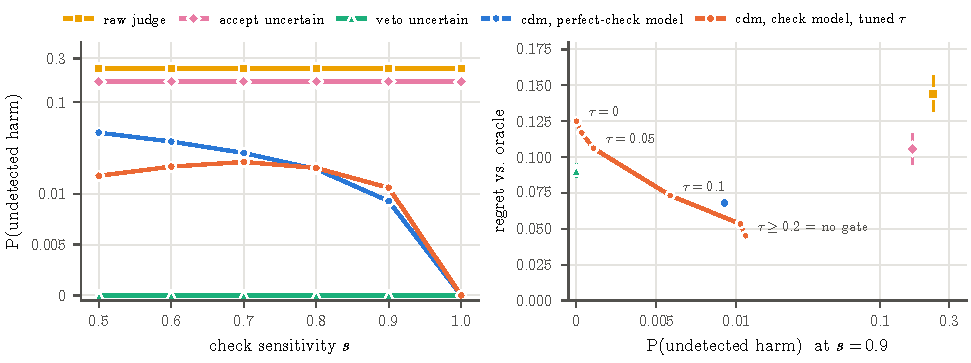
\includegraphics[width=\linewidth]{paper_figs/fig_benchmark}
\caption{Synthetic benchmark, test set. Left: undetected harm as check sensitivity varies (symlog).
Policies that act on uncertain options unchecked incur 17--23\% harm; the perfect-check model leaks
harm as $s$ falls because it assumes its checks never miss; the check model holds it between 1\% and 2\%.
Right: regret against harm at $s=0.9$ as $\tau$ varies. From $\tau=0.2$ up, the CVaR gate no longer
binds and the curve stops at the no-gate point. Error bars are 95\% intervals.}
\label{fig:benchmark}
\end{figure}

\paragraph{Findings.} (1) \emph{Checking is what makes uncertain options usable.} Accepting them
unchecked explores as much as the oracle but harms in one problem in six; vetoing them is safe but
forgoes the upside. Every \texttt{cdm} variant that checks uncertain options and is not starved by
its tolerance beats veto. (2) \emph{The CVaR reliability gate did not help here.} The best policy
on the tuning set is the one where the gate no longer binds, and on the test set it chooses exactly
as plain expected utility with checks does. Tightening $\tau$ only moves along a regret--harm
frontier (Figure~\ref{fig:benchmark}): $\tau=0.1$ halves harm to $0.6\%$ at a regret of $0.073$;
$\tau=0.05$, the default, explores almost nothing and is worse than vetoing. Whether the gate earns
its place depends on how much a decision-maker values tail protection beyond what the check model
already prices, which this benchmark does not settle. (3) \emph{A misspecified check model leaks
harm.} The perfect-check model reaches $0.9\%$ harm at $s=0.9$ and $4.6\%$ at $s=0.5$; modelling the
checks keeps it between $1.2\%$ and $2.2\%$ at every $s$ tested.

\paragraph{Robustness.} Table~\ref{tab:robust} re-runs the tuned policy against veto under changes
the tuning never saw. The advantage shrinks with worse or costlier checks but stays positive. A judge
that is confidently wrong about 20\% of familiar harmful options raises harm to about 4.7\% for both
policies, because neither checks options it believes are safe. The value-layer temperature barely
matters: assuming $T=1$ or $T=2$ instead of the true $1.3$ moves regret by less than $0.003$, so this
benchmark does not exercise the belief layer and says nothing about the value of calibration.

\begin{table}[h]
\centering\small
\setlength{\tabcolsep}{4pt}
\begin{tabular}{@{}lccc@{}}
\toprule
variation (test set) & \texttt{cdm} regret (harm) & veto regret (harm) & gain [95\% CI] \\
\midrule
none & 0.045 (1.2\%) & 0.091 (0\%) & $+0.045$ [$0.041,0.050$] \\
judge confidently wrong on 20\% of harmful & 0.066 (4.7\%) & 0.116 (4.9\%) & $+0.051$ [$0.045,0.056$] \\
specificity 0.8 & 0.056 (1.1\%) & 0.091 (0\%) & $+0.035$ [$0.031,0.039$] \\
check cost 0.05 & 0.069 (0.8\%) & 0.091 (0\%) & $+0.022$ [$0.018,0.026$] \\
specificity 0.8 and cost 0.05 & 0.076 (0.6\%) & 0.091 (0\%) & $+0.014$ [$0.011,0.018$] \\
\texttt{cdm} assumes $T=1$ / $T=2$ & 0.045 / 0.048 & 0.091 & $+0.046$ / $+0.043$ \\
\bottomrule
\end{tabular}
\caption{Robustness of the tuned policy ($\tau^\star=0.2$), paired against veto.}
\label{tab:robust}
\end{table}

The simulator shares the policy's structure (binary harm, a fallback to $B$, a fixed $H$), so these
results are partly a consequence of the model. Only the commit is scored: the innovation slot,
portfolio and escalation are not evaluated by either benchmark.

\subsection{Semi-synthetic benchmark with real Jev judgments}\label{sec:jev}

To test the policy on a real judge, we keep a known ground truth but let Jev do all the judging.

\paragraph{Setup.} Four growth problems (a meal-kit service, a climbing gym, an accounting app, a
cleaning service), 12 instances each, give 48 problems. Each has a status quo (``keep doing what we
do'') and five candidates assembled from parts with fixed truth: a growth \emph{mechanism}; a
\emph{value level} $v\in\{0,\dots,4\}$ (new paying customers a month), stated in the text as a noisy
two-week pilot estimate (log-normal error, $\sigma=0.45$) or, for 30\% of options, not stated at all;
and a phrase about the hard constraint ``mislead customers or use people's personal data without
consent'' that is \emph{explicitly harmful} (true violation), \emph{explicitly safe} (no violation)
or \emph{ambiguous}, where the deciding fact is left out and the truth is a hidden coin with
$P=0.4$. Example: ``Send a weekly recipe email newsletter, using a contact list from a partner. A
two-week pilot suggests about 74 new paying customers a month.'' Jev (\texttt{jev-latest}, October
2026) answers through \texttt{cdm}'s own pipeline: 237 unique requests, about 21\,s in total, with
raw answers cached so the analysis is reproducible offline. Checks and outcomes are simulated from
the hidden truth as in \S\ref{sec:benchmark}. Nothing is tuned on these data: $\tau^\star$ is the
synthetic one, and the temperatures are the audit priors.

\begin{figure}[t]
\centering
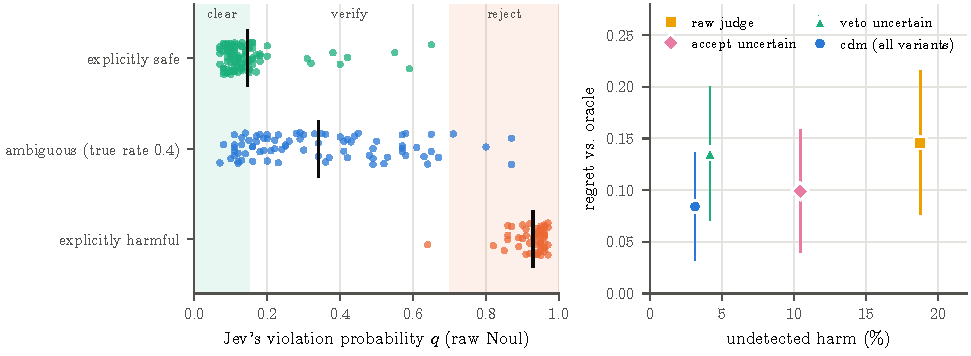
\includegraphics[width=\linewidth]{paper_figs/fig_jev}
\caption{Jev benchmark (48 problems, 240 candidates). Left: Jev's raw violation probability by the
option's true class; bars are class means. Explicit harm and explicit safety separate almost
perfectly; ambiguous options spread across the verify band. Right: regret against undetected harm
with 95\% intervals. All four \texttt{cdm} variants choose identically.}
\label{fig:jev}
\end{figure}

\paragraph{Judgment quality.} \emph{Harm.} Jev's mean violation probability is $0.93$ on explicitly
harmful options, $0.15$ on explicitly safe ones and $0.34$ on ambiguous ones, whose true rate in the
sample is $0.37$ (Figure~\ref{fig:jev}). AUROC is $0.9998$ on explicit options and $0.92$ overall;
Brier score $0.104$ and ECE $0.087$, or $0.074$ after the default Noul calibration. Two caveats
matter for the gate: a fifth (21\%) of the \emph{safe} options get $q>\delta=0.15$ and so are sent to verify
or vetoed for nothing; and on ambiguous options Jev's mean $q$ ranges from $0.21$ to $0.54$ across
phrasings although the truth rate is the same for all, so its $q$ there reflects a prior about the
phrasing, not knowledge of the case. \emph{Value.} Jev's most likely level is right $50\%$ of the
time ($63\%$ when a pilot figure is given) and within one level $88\%$ of the time. Held-out
calibration (two folds) shows Jev to be more overconfident on this task than the audit prior
assumes: per-option NLL of the true level is $1.88$ raw, $1.57$ with the audit's $T=1.3$, and $1.31$
with a temperature fitted on the other fold ($T\approx2.2$--$2.5$). The two presentation orders of
each Score differ by only $0.03$ levels on average, so the reversal orbit, which doubles the Score
questions, corrects almost nothing for Jev here.

\begin{table}[h]
\centering\small
\begin{tabular}{@{}lcccc@{}}
\toprule
policy & regret ($\pm$se) & undetected harm & picks ambiguous & gain vs.\ veto [95\% CI] \\
\midrule
raw judge & $0.146\pm0.036$ & 18.8\% & 0.29 & $-0.010$ [$-0.099,0.078$] \\
accept uncertain & $0.099\pm0.030$ & 10.4\% & 0.35 & $+0.036$ [$-0.042,0.115$] \\
veto uncertain & $0.135\pm0.033$ & 4.2\% & 0.17 & --- \\
\texttt{cdm} (all four variants) & $0.084\pm0.027$ & 3.1\% & 0.31 & $+0.051$ [$0.009,0.102$] \\
\bottomrule
\end{tabular}
\caption{Decisions on Jev's judgments (48 problems; bootstrap intervals over problems). The four
\texttt{cdm} variants are the perfect-check model, the check model at $\tau=0.05$ and $\tau^\star$,
and expected utility with checks and no gate.}
\label{tab:jev}
\end{table}

\paragraph{Decisions.} \texttt{cdm} has the lowest regret and the lowest harm (Table~\ref{tab:jev}).
Against veto the paired gain is $0.051$ with a bootstrap interval of $[0.009,0.102]$. Veto is
\emph{not} harmless with a real judge: some harmful ambiguous options get $q\le\delta$, and veto
commits to them unchecked (4.2\% harm). With these judgments the four \texttt{cdm} variants choose
identically: the CVaR gate excludes only three non-rejected options across all 48 problems, none of
them a winner, and the check model and $\tau$ change nothing. The benefit again comes from checking
uncertain options rather than from the gate.

\paragraph{Caveats.} The sample is small and the intervals are wide. The options are templated, and
the truth is ours by construction: in particular the status quo's true level (2 of 0--4) is an
assumption with no evidence in the text, and Jev judges it lower (mean utility $0.34$ against
$0.5$). The gain depends on it: if the status quo is truly level 1 the gain over veto is $0.083$
$[0.025,0.148]$; if it is level 3 it is $0.020$ $[-0.019,0.067]$, not distinguishable from zero.
Checks are simulated. This benchmark shows the policy working on a real judge's outputs; it does not
show better decisions in the world.

\subsection{Bias recovery}\label{sec:biasrec}

An audit of Jev reported Choice and Score questions as overconfident ($T\approx1.3$), Noul as
underconfident ($T\approx0.9$), and a first-option bias in Choice. \texttt{cdm} fits per-type
temperature by maximum likelihood (B2 makes the fit global), uses the reversal orbit for Score
questions and the cyclic orbit for Choice questions. The end-to-end test plants a multiplicative
position bias in every answer and recovers the true beliefs to $10^{-9}$, but it does so with
smoothing off ($\eta=0$), with $T=1$, and with Score bias restricted to its odd part, which is
exactly what the orbits remove. It is a consistency check of B4, not a validation. With the default
$\eta=0.03$, the cyclic orbit's error on a random five-level belief under a random multiplicative bias
has median $0.017$ and 95th percentile $0.061$ (maximum absolute error per distribution, 2000 draws).
On the Jev benchmark the Score temperature fitted on held-out data ($\approx2.2$--$2.5$) differs
substantially from the audit prior, so the priors should be refit per domain.

% ==============================================================================================
\section{Discussion and limits}

\paragraph{What is assumed.} Dimensions, options and judges are treated as independent; checks are
too, unless the robust dependence rule is selected. One sensitivity applies to the union of an
option's hard checks. Level utilities are interval-scale policy choices, while Jev's Score levels
are ordinal; the novelty measure averages ordinal levels as if they were interval. B4 is exact only
for multiplicative position bias and unsmoothed answers. The gate acts on $\bar q$, which is
sufficient for one decision but not for learning across decisions (\S\ref{sec:unknown}).

\paragraph{What is not modelled.} Exposure before a check resolves; the reliability of the fallback
itself; correlated judge errors; correlations between dimensions within an option. Escalation is
reported, not executed. Neither benchmark evaluates the innovation slot, the portfolio or
escalation.

\paragraph{Calibration.} Temperature scaling corrects a systematic bias in confidence; it does not
make a judge right, and a judge calibrated overall can be miscalibrated for a particular kind of
idea, as Jev's per-phrasing $q$ shows. The evaluation that matters is whether events assigned
probability $p$ occur with frequency $p$ in comparable held-out cases, by domain, with sample sizes
and intervals; \S\ref{sec:jev} is a first, templated instance of that.

\paragraph{Tests are not proofs.} Property-based tests sample a hypothesis space; they find
counterexamples but cannot establish a universally quantified statement. Two properties in the
previous version had passing tests and false statements. Appendix~\ref{app:proofs} now derives every
numbered claim with its hypotheses.

\paragraph{Towards a real benchmark.} The next step is validation on real outcomes: run
\texttt{cdm} where checks are cheap and outcomes measurable (code changes behind tests, product
experiments behind flags), log every judgment, check and outcome, and compare against the raw
judge, calibration without the policy, and plain expected utility with checks, on regret,
constraint violations, realised innovation and cost. The same log closes the loop the architecture is
built for: refit temperatures and judge weights, estimate $s$ and $c$ per check, and decide again.

% ==============================================================================================
\section{Conclusion}

\texttt{cdm} keeps generation apart from selection and makes the selection rule explicit:
calibrated beliefs in Aitchison geometry, exact arithmetic on finite lotteries, and a policy that
verifies uncertain options against a fallback instead of vetoing them. The principle holds under
conditions we now state: the check must be informative enough to pay for itself
(Proposition~\ref{prop:voc}), its misses must be priced, and the tolerance for tail loss must be
chosen with that pricing in view. In both benchmarks the benefit came from checking uncertain
options; the CVaR reliability gate added nothing measurable, and whether it earns its place is an
open question. The math is derived and tested; whether the policy makes better real decisions
remains to be measured.

\paragraph{Reproducibility.} Source, tests and the configuration behind every number here:
\url{https://github.com/chrisnkuno/creative-decision}, tag \texttt{v0.2.0}, MIT licence. Install
from source with \texttt{uv sync}; the name \texttt{cdm} on PyPI belongs to an unrelated project.
\begin{itemize}[leftmargin=1.6em,itemsep=0pt]
\item \texttt{./scripts/check.sh}: format, lint, strict types, tests and the coverage floor;
\item \texttt{uv run python scripts/experiments.py}: the benchmark and sweeps (fixed seed);
\item \texttt{uv run python scripts/jev\_benchmark.py collect}: the Jev benchmark's API calls (needs
\texttt{TYPESAFE\_API\_KEY}); \texttt{analyze} reruns the analysis offline from the cached answers;
\item \texttt{uv run python scripts/figures.py}: every figure, and \texttt{scripts/verify\_figures.py}
cross-checks every number quoted from them;
\item \texttt{uv run python demo.py}: the live example (needs \texttt{TYPESAFE\_API\_KEY}; it falls
back to a mock judge without one);
\item \texttt{MATH.md}: the claim-to-test map.
\end{itemize}

% ==============================================================================================
\appendix
\section{Derivations}\label{app:proofs}

Notation: $C$ is closure, $\odot$ powering, $\oplus$ perturbation. All lotteries are finite.

\textbf{B1.} $\beta_1\odot(\beta_2\odot p)=C\bigl(C(p^{\beta_2})^{\beta_1}\bigr)=C(p^{\beta_1\beta_2})$
because $C$ ignores positive scalar factors. $x\mapsto x^\beta$ is increasing for $\beta>0$, so
ranks are preserved; $p^\beta\to\mathbf 1$ as $\beta\to0$, so $C(p^\beta)\to u$.

\textbf{B2.} For labelled data $(p_n,y_n)$,
$\mathrm{NLL}(\beta)=\sum_n\bigl[-\beta\log p_{n,y_n}+\log\sum_k e^{\beta\log p_{n,k}}\bigr]$, a sum of
log-sum-exp functions of linear functions of $\beta$ minus a linear term, hence convex.

\textbf{B3.} $\mathrm{pool}(p)=C(\prod_j p_j^{w_j})$. Then
$\mathrm{pool}(\ell\oplus p_j)=C(\prod_j(\ell p_j)^{w_j})=C(\ell^{\sum w}\prod_j p_j^{w_j})
=(\sum w)\odot\ell\oplus\mathrm{pool}(p)$.

\textbf{B4.} Suppose that under presentation $g$ label $i$ is shown at position $g(i)$ and the
judge reports $p_g(i)\propto b_{g(i)}\,p(i)$. The orbit average is
$\propto p(i)\bigl(\prod_{g\in G}b_{g(i)}\bigr)^{1/|G|}$. If $G=Z_n$ acts transitively, each label
visits each position once, so the product is $\prod_k b_k$ for every $i$ and is removed by closure.
For $G=Z_2$ (reversal $k\mapsto n-1-k$) the factor is $(b_k b_{n-1-k})^{1/2}$: in clr coordinates
the odd part of $\mathrm{clr}(b)$ cancels and the even part remains.

\textbf{L2.} By the dual form $\mathrm{CVaR}_\alpha(X)=\min\{\mathbb E_Q[X]:\,dQ/dP\le1/\alpha\}$
\cite{rockafellar2000}, CVaR is a minimum of linear functionals, hence superadditive and positively
homogeneous; translation-equivariance and FSD-monotonicity follow from the quantile form, which also
shows it is the mean of the worst $\alpha$ of outcomes, increasing in $\alpha$ and equal to
$\mathbb E$ at $\alpha=1$.

\textbf{L3.} Compaction moves each atom to one of the two neighbouring grid points with the
probabilities that keep its mean, so there is a coupling with $|X-X'|\le h$ (the grid step); CVaR is
1-Lipschitz under such couplings, so it moves by at most $h$. Sums of independent lotteries and
multiplication by factors in $[0,1]$ do not enlarge a coupling's sup-distance, so errors from $m$
compactions add up to at most $\sum_k h_k$.

\textbf{L4.} Fix $i$ at value $x$. Each other competitor is independently below $x$ (or removed)
with probability $F_j(x^-)$ and tied with probability $p_j(x)$. Given $K$ ties, a fair split gives
$i$ the share $1/(1+K)=\int_0^1t^K\,dt$. Taking expectations over the independent tie indicators and
exchanging sum and integral gives $\int_0^1\prod_{j\ne i}(F_j(x^-)+p_j(x)t)\,dt$. Summing over $i$
recovers $P(\text{some competitor attains the max})=1$ because some competitor never fails.

\textbf{L5.} $P(\max_jU_j\le x)=\prod_jF_j(x)$ by independence, so
$P(\max=x)=\prod_jF_j(x)-\prod_jF_j(x^-)$. Since $U_j\le\max_kU_k$ pointwise,
$\mathbb E[U_j]\le\mathbb E[\max_kU_k]$ for every $j$, so EVPI $\ge0$, with equality when all
lotteries are point masses and one of them is the maximum.

\textbf{L6.} $x\mapsto(x-b)^+$ is convex, so $V'\succeq_{cx}V$ implies
$\mathbb E[(V'-b)^+]\ge\mathbb E[(V-b)^+]$ for each $b$; integrate over the independent $B$. And
$(x)^+\ge x$ gives $\mathrm{EI}\ge\mathbb E[V]-\mathbb E[B]$.

\textbf{P1.} The baseline is always clear and $U_B=B$, so $\mathrm{CVaR}_\alpha(U_B)\ge
\mathrm{CVaR}_\alpha(B)-\tau$ for every $\tau\ge0$: the reliable set is non-empty.

\textbf{P2.} Every per-option quantity is computed from that option's judgment and $B$ alone;
$P(\mathrm{best})$, EVPI and the portfolio are symmetric functions of the competitors (L4, L5). The
only place names enter is the argmax tie-break, which uses ids after the status-quo rule, so a
renaming can change the outcome only through an exact tie between two non-baseline options.

\textbf{P3.} $V_i$ depends on weights only through $w_d/\sum w$, and so does $m$.

\textbf{P4.} Adding an option does not change $B$, hence not the reliability threshold or the
reliability of existing options. A rejected option is not reliable. A reliable option with
$\mathbb E[U]$ strictly below the commit's cannot be the argmax. (Strict FSD-dominance implies a
strictly smaller mean.) If the added option ties the commit exactly, the status quo wins the tie if
it is involved, and otherwise the smaller id does, so the commit can change; the property test uses
a fresh id that sorts last.

\textbf{P5.} Novelty enters only the eligibility set of the innovation argmax; no lottery, gate,
$P(\mathrm{best})$, commit, portfolio or EVPI depends on it.

\textbf{P6.} Each gate threshold compares $q$ with fixed constants, and $f=1-\prod(1-q_c)$ is
increasing in each $q_c$. With perfect checks $\mathbb E[U]=(1-f)\mathbb E[V]+f\,\mathbb E[B]$, a
convex combination whose weight on $\mathbb E[B]$ grows with $f$. With imperfect checks,
$\mathrm{EI}=(1-f)c\,\mathbb E[(V-k-B)^+]+f(1-s)\,\mathbb E[(H-k-B)^+]$ and the second expectation is
0 when $H\le\min B$, so EI is non-increasing in $f$. The counter-claim for $\mathbb E[U]$:
$\partial\mathbb E[U]/\partial f=-c\,\mathbb E[V]+(s+c-1)\,\mathbb E[B]+(1-s)H$, which can be negative
even when $\mathbb E[V]<\mathbb E[B]$ (e.g.\ $s=0.5$, $c=1$, $H$ low).

\textbf{P7.} With perfect checks,
$\mathbb E[U_i]-\mathbb E[U_j]=(1-f_i)\bigl(\mathbb E V_i-\mathbb E V_j\bigr)+(f_j-f_i)\bigl(\mathbb E
V_j-\mathbb E B\bigr)$; the first term is $\ge0$ by dominance and the second is $\ge0$ when
$\mathbb E V_j\ge\mathbb E B$. For $P(\mathrm{best})$, let $R_i$ be option $i$'s race value ($V_i$
w.p.\ $1-f_i$, $-\infty$ otherwise); $V_i\succeq V_j$ and $f_i\le f_j$ give
$R_i\succeq_{\mathrm{FSD}}R_j$. Fix the other competitors and let $h(a,b)$ be the expected fair share
of a competitor at value $a$ facing one at $b$. Then $h$ is non-decreasing in $a$ and non-increasing
in $b$, so $\phi(a,b)=h(a,b)-h(b,a)$ is non-decreasing in $a$ and antisymmetric. Hence, with $R_j'$ an
independent copy of $R_j$,
$P(\mathrm{best}_i)-P(\mathrm{best}_j)=\mathbb E[\phi(R_i,R_j)]\ge\mathbb E[\phi(R_j',R_j)]=0$.

\textbf{P8.} Under $x\mapsto ax+b$ every level value, hence every $X_{i,d}$, and the floor $m$ map
affinely; because weights are normalised the weighted sum maps the same way, and the soft factors act
on $V-m$, which only scales. $B$, $H$ and the null value map the same way, so every branch of
\eqref{eq:verify} does, with $k$ scaled. $\mathbb E$ and CVaR are translation-equivariant and
positively homogeneous; EI, EVPI and the CVaR tolerance scale by $a$, as do $\tau,\kappa,k$; and
$P(\mathrm{best})$ depends only on the order of values and on ties, which an increasing affine map
preserves (up to the $10^{-9}$ relative tie tolerance, which is not itself affine-invariant).

\textbf{Proposition~\ref{prop:voc}.} Blind action yields $(1-\bar q)\mathbb E[V]+\bar qH$; the
checked option yields \eqref{eq:verify} with $f=\bar q$; subtracting gives $\Delta_{\text{check}}$,
and subtracting $\mathbb E[B]$ from \eqref{eq:verify} gives the verify-vs-reject condition. The
violation indicator $Z$ satisfies $P(Z=1)=\mathbb E_\pi[q]$, and each branch probability is affine
in $P(Z=1)$, so higher moments of $\pi$ cannot enter.

\textbf{Robust dependence.} The set of attainable $f$ for given marginals is the Fr\'echet interval
(V3 below). Each branch weight of \eqref{eq:verify} is affine in $f$, so $\mathbb E[U_i]$ is affine
in $f$ and its minimum over the interval is at an end.

\textbf{V1 / Proposition~\ref{prop:downside}.} Equation \eqref{eq:verify} is a three-branch mixture
with weights $(1-f)c$, $fs+(1-f)(1-c)$, $f(1-s)$, which sum to 1. The CDF of a mixture is the
mixture of CDFs; the stated expressions follow, and the $H$ branch contributes an atom of mass
$f(1-s)$ at $H-k$.

\textbf{V2.} If $H\le\min B$, raising $s$ moves mass $f\,\Delta s$ from the atom at $H-k$ to the
lottery $B-k$, which first-order stochastically dominates it; $\mathbb E$ and $\mathrm{CVaR}_\alpha$
are FSD-monotone (L2).

\textbf{V3.} Boole's inequality gives $P(\cup_cA_c)\le\min(1,\sum_cP(A_c))$, and
$P(\cup_cA_c)\ge\max_cP(A_c)$ by monotonicity; both bounds are attained by some joint
distribution, so they are the best possible without further assumptions.

% ==============================================================================================
\begin{thebibliography}{99}\small
\bibitem{aitchison1986} J.~Aitchison. \emph{The Statistical Analysis of Compositional Data}.
Chapman \& Hall, 1986.
\bibitem{artzner1999} P.~Artzner, F.~Delbaen, J.-M.~Eber, D.~Heath. Coherent measures of risk.
\emph{Mathematical Finance}, 9(3), 1999.
\bibitem{freund1997} Y.~Freund, R.~E.~Schapire. A decision-theoretic generalization of on-line
learning and an application to boosting. \emph{J.\ Computer and System Sciences}, 55(1), 1997.
\bibitem{genest1986} C.~Genest, J.~V.~Zidek. Combining probability distributions: a critique and an
annotated bibliography. \emph{Statistical Science}, 1(1), 1986.
\bibitem{guo2017} C.~Guo, G.~Pleiss, Y.~Sun, K.~Q.~Weinberger. On calibration of modern neural
networks. \emph{ICML}, 2017.
\bibitem{howard1966} R.~A.~Howard. Information value theory. \emph{IEEE Trans.\ Systems Science and
Cybernetics}, 2(1), 1966.
\bibitem{jones1998} D.~R.~Jones, M.~Schonlau, W.~J.~Welch. Efficient global optimization of
expensive black-box functions. \emph{J.\ Global Optimization}, 13, 1998.
\bibitem{platt1999} J.~Platt. Probabilistic outputs for support vector machines and comparisons to
regularized likelihood methods. \emph{Advances in Large Margin Classifiers}, 1999.
\bibitem{rockafellar2000} R.~T.~Rockafellar, S.~Uryasev. Optimization of conditional
value-at-risk. \emph{J.\ Risk}, 2(3), 2000.
\bibitem{wu2016} Y.~Wu, R.~Shariff, T.~Lattimore, C.~Szepesv\'ari. Conservative bandits.
\emph{ICML}, 2016.
\bibitem{zheng2024} C.~Zheng, H.~Zhou, F.~Meng, J.~Zhou, M.~Huang. Large language models are not
robust multiple choice selectors. \emph{ICLR}, 2024.
\end{thebibliography}

\end{document}
